\chapter{Конструкторский раздел}
В данном разделе представлены схемы реализуемых алгоритмов и их модификации.
\section{Матричные итерационные алгоритмы}
На рисунке \ref{fig:l-iter-matrix} изображена схема алгоритма нахождения расстояния Левенштейна итерационно  с использованием матрицы расстояний.
На рисунке \ref{fig:d-iter-matrix} изображена схема алгоритма нахождения расстояния Дамерау -- Левенштейна итеративно  с использованием матрицы расстояний.
\section{Модификация матричных алгоритмов}
Мемоизация - это прием сохранения промежуточных результатов, которые могут еще раз понадобиться в ближайшее время, чтобы избежать их повторного вычисления. 
Матричный алгоритм нахождения расстояния Дамерау -- Левенштейна может быть модифицирован, используя мемоизацию -- достаточно инициализировать матрицу значением $\infty$, которое будет рассмотрено в качестве флага.
На рисунке \ref{fig:l-recur-matrix} изображена схема алгоритма, использующая этот прием.
\section{Рекурсивные алгоритмы}
На рисунке \ref{fig:d-recur} изображена схема рекурсивного алгоритма  нахождения расстояния Дамерау -- Левенштейна.
\newpage 
\begin{figure}[h!]
	\begin{center}
		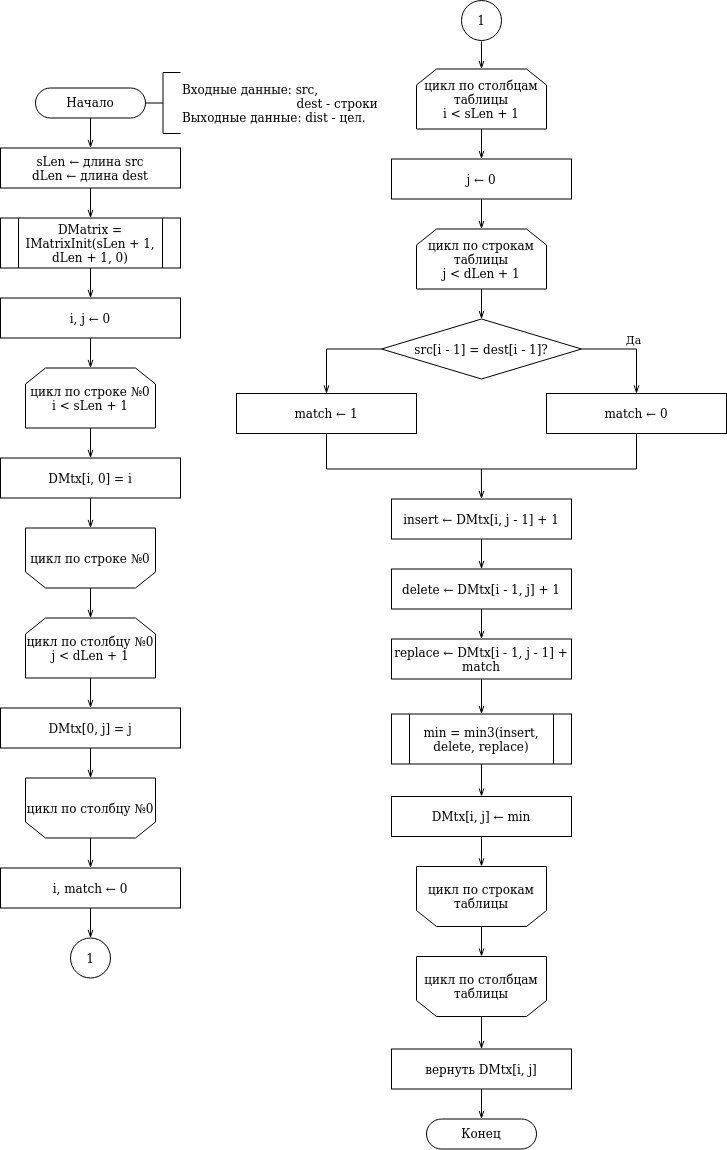
\includegraphics[scale=0.6]{./assets/leven-matrix-iter.png}
	\end{center}
	
	\caption{Схема итерационного алгоритма расстояния Левенштейна с заполнением матрицы расстояний}
	\label{fig:l-iter-matrix}
\end{figure}


\begin{figure}[h!]
	\begin{center}
		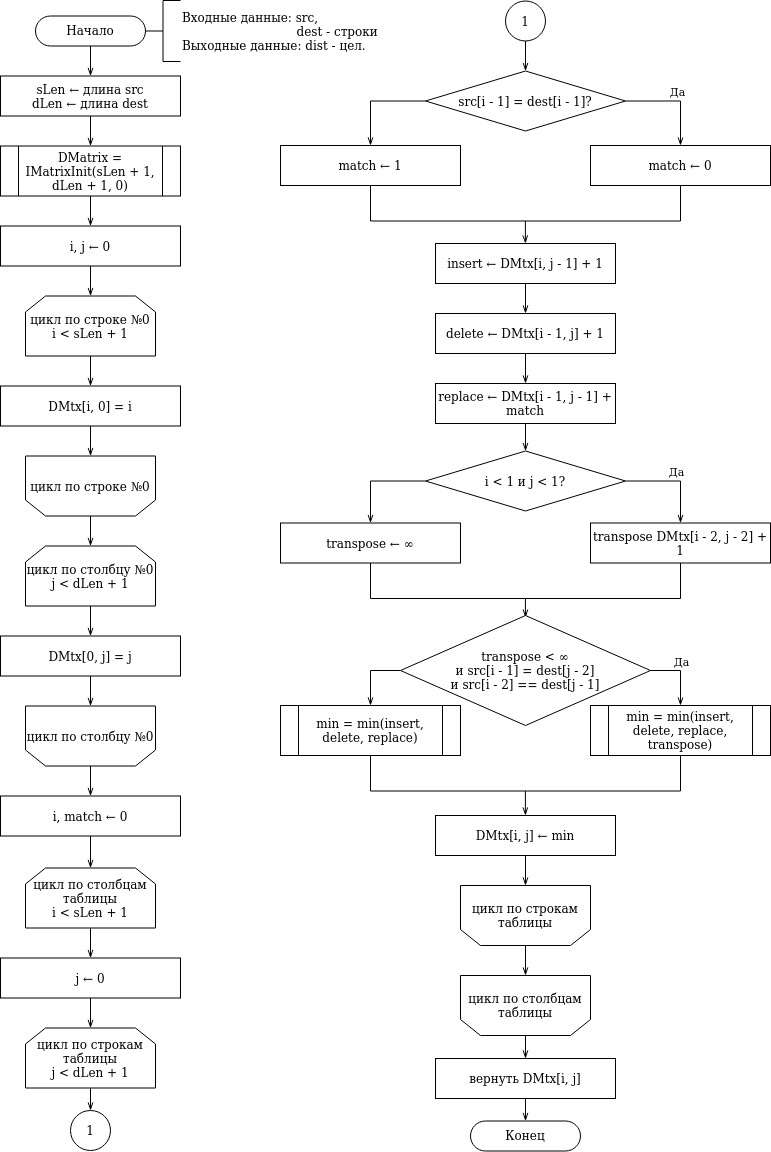
\includegraphics[scale=0.6]{./assets/d-leven-iter.png}
	\end{center}
	
	\caption{Схема итерационного алгоритма расстояния Дамерау -- Левенштейна с заполнением матрицы расстояний}
	\label{fig:d-iter-matrix}
\end{figure}

\begin{figure}[h!]
	\begin{center}
		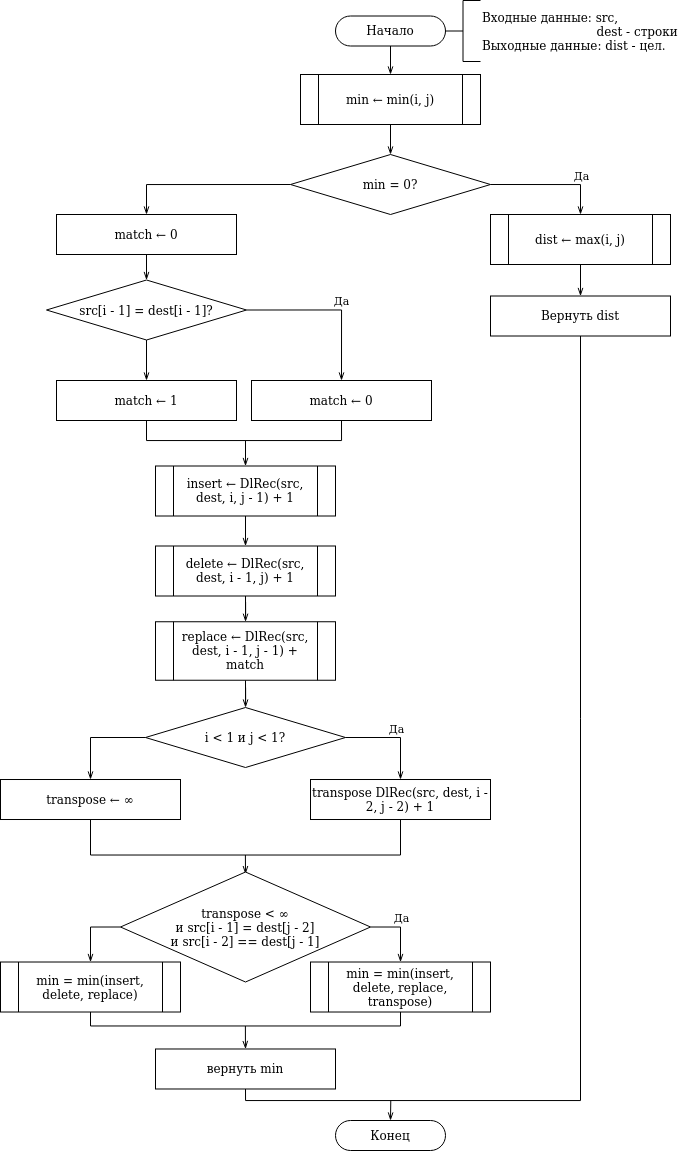
\includegraphics[scale=0.6]{assets/d-leven-recursive.png}
	\end{center}
	
	\caption{Схема рекурсивного алгоритма расстояния Дамерау - Левенштейна}
	\label{fig:d-recur}
\end{figure}

\begin{figure}[h!]
	\begin{center}
		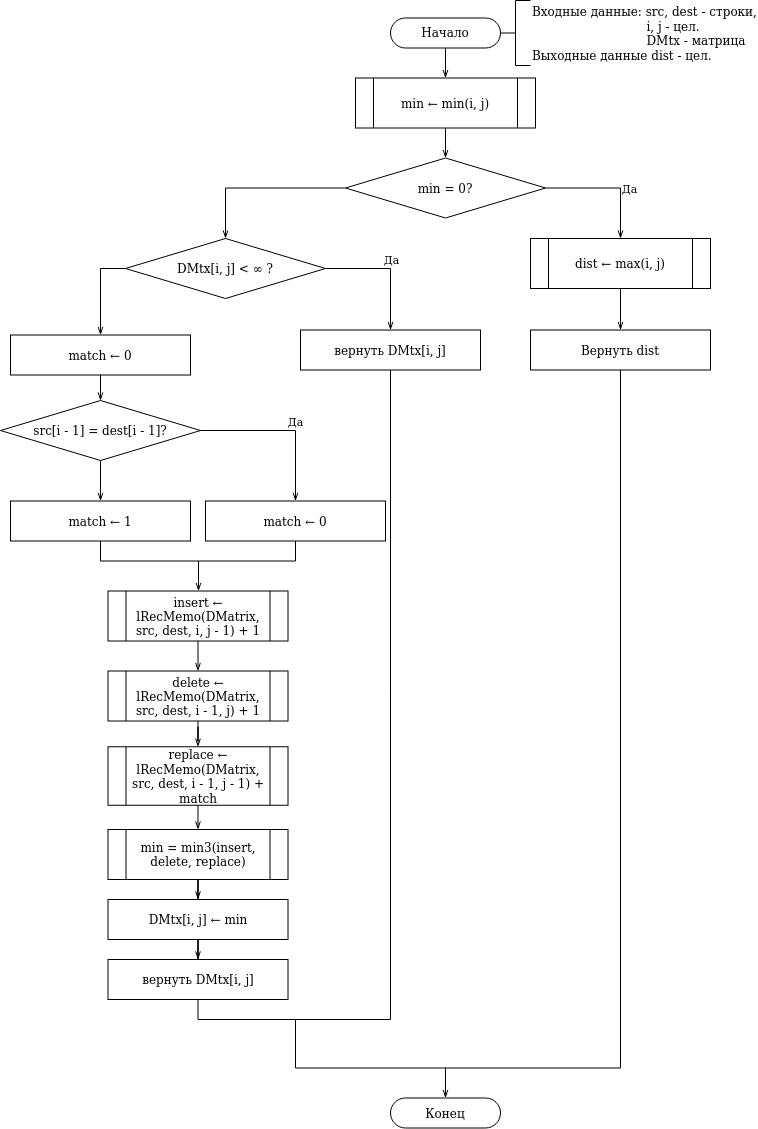
\includegraphics[scale=0.6]{./assets/leven-matrix-memo.png}
	\end{center}
	
	\caption{Схема рекурсивного алгоритма расстояния Левенштейна с мемоизацией}
	\label{fig:l-recur-matrix}
\end{figure}



\section{Вывод}
На основе формул и теоретических данных, полученных в аналитическом разделе, были спроектированы схемы алгоритмов.